\documentclass[12pt]{article}
\usepackage[utf8]{inputenc}
\usepackage{amsmath}
\usepackage{amsfonts}
\usepackage{amssymb}
\usepackage{graphicx}
\usepackage{physics}
\usepackage{float} 
\usepackage[margin=1in]{geometry}
\usepackage{enumitem}
\usepackage{breqn}
\usepackage{soul,color}
\usepackage{blindtext}
\usepackage{mathtools}
\usepackage{verbatim}
\begin{document}
\title{ Vertex Model Calculations \\ {\normalsize Adjusting Box Size}}
\author{Avik Mondal}
\maketitle 
\tableofcontents
\section{Citation}
Citation: Carolina Baruffi. Application of an Overdamped Langevin Dynamics to the study of microstructural evolutions in crystalline materials. Engineering Sciences [physics]. SORBONNE UNIVERSITE, 2018.
English.\\ 
The formalism used in this set of notes came from this paper. 

\section{Introduction to Brownian Dynamics}
Because we are modeling an infinite tissue with periodic boundary conditions, we want to be able to maintain an NPT (number of d.o.f, pressure, and temperature stay constant) ensemble.  If we do not keep the pressure constant, growing cells can cause build ups of stress that would emulate finite size effects. Additionally, we want to keep our tissue in an equilibrium regime. If we allow the tissue to grow, we then have to control the pressure in order to have access to accurate calculations of thermodynamics potentials (in our case, enthalpy) \\ \\
The main question is how to accurately maintain an NPT ensemble. I have found that a Brownian dynamics approach is best. The basic equation for these dynamics:

\begin{center}
\begin{equation}
\label{eqn: browniandynamics}
\pdv{x_i}{t} = -\nu_i \pdv{F}{x_i} + B_i \eta_i(t)
\end{equation}
\end{center}
Here, the subscript "i" is an index for all the particle degrees of freedom (or in our case, vertex degrees of freedom). $F$ refers to the relevant thermodynamic potential of the system. In our case, because we are trying to maintain a constant pressure, enthalpy (H) is the appropriate potential. $\eta$ is a stochastic term. $B_i$ is the amplitude of the noise. This dynamical equation is the overdamped limit of the more general Langevin dynamics. This is appropriate for the vertex model since it generally assumes that flow in the system has a low Reynold's number. \\
We assume the noise terms are independent and represent white Gaussian noise:
\begin{center}
\begin{equation}
\label{eqn: noiseconditions}
\expval{\eta_i(t)} = 0, \hspace{1cm}
\expval{\eta_i(t) \eta_j(t')} = \delta_{ij} \delta(t-t')
\end{equation}
\end{center}
We consider the case in which the noise amplitudes are proportional to the square root of the mobility terms, such that:
\begin{center}
\begin{equation}
B_i^2 = 2 \alpha \nu_i
\end{equation}
\end{center}
$\alpha$ is the proportionality constant that we can determine with phenomenology. Equation \ref{eqn: browniandynamics} is equivalent to the following Fokker-Planck equation:
\begin{center}
\begin{equation}
\label{eqn: fokkerplanck}
\dv{P(\{x_i^n\})}{t} = \sum\limits_i \pdv{x_i} \Big[\nu_i \pdv{E}{x_i}P(\{x_i^n\}  )\Big] + 2 \sum\limits_i \pdv{x_i^2} \big[(4 \alpha \nu_i)^2 P(\{x_i^n\})\big]
\end{equation}
\end{center}

Assuming boundary conditions where:
\begin{center}
\begin{equation}
\lim_{x_i\to \infty} P(\{x_i^n\}) = 0
\end{equation}
\end{center}
and restricting to integrable probability densities , then we expect a fixed point of the Fokker-Planck equation to be:
\begin{center}
\begin{equation}
\label{eqn: fp}
P_{fp}(\{x_i^n\}) = A \exp\bigg(-\cfrac{E({x_i})}{\alpha}\bigg)
\end{equation}
\end{center} 
To normalize:
\begin{center}
\begin{equation}
\label{eqn: A}
A^{-1} = \int \exp \bigg(-\cfrac{E({x_i})}{\alpha}\bigg) \prod\limits_i d x_i
\end{equation}
\end{center}
Additionally, we can see that to recover thermal equilibrium (as we would expect), we can say 
\begin{center}
\begin{equation}
\label{eqn: alpha}
\alpha = k_B T
\end{equation}
\end{center}
Maintaining this Boltzmann distribution is an important part of this dynamic process. In our case, we do not have to think to much about the noise because we are not giving our vertices stochastic dynamics (so we are in the \ul{overdamped, $T = 0$} limit).
\section{NPT ensemble}
To keep the pressure constant, we have to allow the box size to adjust. To do this, we have to formally introduce degrees of freedom and dynamics that will allow us to control the box length and width.  Instead of using the length and width of the box as Meryl does, we will use a deformation gradient. \\ \\

We can describe the box as the parallelogram defined by two non-collinear vectors $\vb{L_1}(t)$ and $\vb{L_2}(t)$. We assume then that our tissue deforms homogeneously, so then we can describe the change in shape using a deformation gradient $F(t)$ such that:
\begin{center}
\begin{equation}
\label{eqn9}
(L_\alpha)_i(t) = F_{ij} (L_\alpha(t = 0))_j,\hspace{1cm} \alpha = 1,2
\end{equation}
\end{center} 
With this, we can introduce a new tensor to make our calculations more convenient:
\begin{center}
\begin{equation}
\label{eqn10}
L = 
\begin{pmatrix}
|\vb{L_1}(0)| & 0\\
0 & |\vb{L_2}(0)|\\  
\end{pmatrix}
\end{equation}
\end{center}
This is a tensor containing the initial lengths of the box dimensions. We can now use this and $F$ to relate the scaled coordinates to the unscaled coordinates:
\begin{center}
\begin{equation}
\label{eqn: coords}
\tilde{x_i} = (L_{ik}^{-1} F_{kj}^{-1})x_j
\end{equation}
\end{center}
and additionally $A(t) = A_0 \det F$, where $A$ is the area and $A_0$ is the initial area of the box. This is effectively saying that $\tilde{x_i} = \frac{x_i} {L_i(t)}$. Note that for our case, we want our box to stay rectangular. The easiest way to make this happen is to impose the condition that $F$ remain diagonal. \\ \\
With this, we can introduce a new energy for our box:
\begin{center}
\begin{equation}
\label{eqn: boxenergy}
U_{box}(F) = A_0 (\det(F)) \tr{\sigma_{ext}}
\end{equation}
\end{center}
where $A_0 = (\vb{L_1} (0)\cross \vb{L_2} (0)) \cdot \vu{z}$. In our specific case where the vectors never shear, we can say $A_0 = L_{xx} L_{yy}$. In the case where we want hydrostatic external (compressive) pressure.
\begin{center}
\begin{equation}
\label{eqn: hydrostatic_stress}
(\sigma_{ext})_{ij} = \frac{1}{2} p \delta_{ij} 
\end{equation}
\end{center}
The full enthalpy of our box is then:
\begin{center}
\begin{equation}
\label{eqn: enthalpy}
H(\{\tilde{x_i}^n\}, F) = E_0(\{\tilde{x_i^n}\}) - p A_0 (\det(F))
\end{equation}
\end{center}
$E_0$ is the potential energy of the vertex model. From this we can identify the dynamics:
\begin{center}
\begin{equation}
\label{eqn: dyn}
\pdv{\tilde{x_i^n}}{t} = -\nu \fdv{H}{\tilde{x_i^n}}\bigg\vert_{F}, \hspace{2cm} \pdv{F_{\alpha \beta}}{t} = -\mu \fdv{H}{F_{\alpha\beta}}\bigg\vert_{\tilde{x_i^n}}
\end{equation}
\end{center}
Before I go on, I should say that the enthalpy above reduces to Boltzmann's distribution (outside of $T = 0$) when you add an extra term to this enthalpy. The following enthalpy is best to use:
\begin{center}
\begin{equation}
\bar{H} = H - N k_B T \log(V_0 \det(F))
\end{equation}
\end{center}
The explanation for this is in the paper cited at the top.

\textbf{June 1 Addendum}. It has become necessary to consider an external stress that is not just a hydrostatic pressure. Thus, the applied stress tensor looks like:

\begin{center}
\begin{equation}
\label{eqn: hydrostatic_stress}
(\sigma_{ext})_{ij} = \frac{1}{2}\bigg( p \delta_{ij} + \sigma^{(tl)}_{ij}\bigg)
\end{equation}
\end{center}

where I have introduced a traceless component to the stress. In this case, we can adjust calculations below by replacing $p$ with $p + \sigma^{(tl)}_{ij}$, with the appropriate indices plugged in. The traceless portion of the stress is diagonal.
\section{Calculation of the Dynamics} 
The dynamics of the scaled coordinates reduce pretty simply to:
\begin{center}
\begin{equation}
\pdv{\tilde{x_i^n}}{t} = -\nu \pdv{E_0}{\tilde{x_i^n}}
\end{equation}
\end{center}
However, the model is currently coded so that using unscaled coordinates as a parameter may be more convenient. Then, we can use the chain rule to find out what the dynamics of this would be:
\begin{center}
\begin{equation}
\pdv{\tilde{x_i^n}}{t} = \pdv{\tilde{x_i^n}}{x_i^n}\bigg\vert_{L_i} \pdv{x_i^n}{t} + \pdv{\tilde{x_i^n}}{L_{i}}\bigg\vert_{x_i^n} \pdv{L_{i}}{t} = \pdv{x_i^n}{t} \frac{1}{|L_i(t)|} - \frac{x_i^n}{L_{i}^2} \pdv{L_{i}}{t}
\end{equation}
\end{center}
These dynamics are a bit messier, but this is quite similar to what already exists in the vertex model. For the other side of the equation: 
\begin{center}
\begin{equation}
\pdv{x_i^n}{t} \frac{1}{L_i(t)} - \frac{x_i^n}{L_{i}^2}\pdv{L_{i}}{t} = -\nu\pdv{E_0}{\tilde{x_i^n}}\bigg\vert_F = -\nu \pdv{E_0}{x_i^n} \pdv{x_i^n}{\tilde{x_i^n}}\bigg\vert_{F}
\end{equation}
\end{center} 
We don't have an extra derivative with respect to $F_{\alpha\beta}$ on the right hand side because for this equation, $F_{\alpha\beta}$ is held constant. Then, we can simplify and say:
\begin{center}
\begin{equation}
\pdv{x_i^n}{t}  = -\nu L_i(t)^2\pdv{E_0}{x_i^n} + \frac{x_i^n}{L_{i}} \pdv{L_{i}}{t}
\end{equation}
\end{center} 
Then, we need the dynamics of the deformation gradient to fully understand those of the coordinates. \\ \\
The dynamics of the deformation gradient are a bit messier:
\begin{center}
\begin{equation}
\label{eqn: dfdt}
\pdv{F_{\alpha \beta}}{t} = -\mu\pdv{F_{\alpha\beta}}\bigg\vert_{\tilde{x^n}}\bigg[ E_0 + p A_0(\det(F))\bigg]
\end{equation}
\end{center}
Note that $\pdv{\det{F}}{F} = \det{F} F^{-T}$.
\begin{center}
\begin{equation}
\label{eqn: dfdtstep1}
\pdv{F_{\alpha \beta}}{t} = -\mu\bigg\{\pdv{E_0}{F_{\alpha\beta}}\bigg\vert_{\tilde{x^n}} + p A(t) F_{\alpha\beta}^{-T}\bigg\}
\end{equation}
\end{center}
Use chain rule, but keep the constant scaled coordinates in mind:
\begin{center}
\begin{equation}
\label{eqn: dfdtchainrule}
\pdv{F_{\alpha \beta}}{t} = -\mu\bigg\{\sum\limits_{n,i} \pdv{E_0}{x_i^n} \pdv{x_i^n}{F_{\alpha\beta}}\bigg\vert_{\tilde{x}^n} + p A(t) F_{\alpha\beta}^{-T}\bigg\}
\end{equation}
\end{center}
Now, using Eqn \ref{eqn: coords}, we can see that:
\begin{center}
\begin{equation}
\pdv{x_i^n}{F_{\alpha \beta}}\bigg\vert_{\tilde{x}_i^n} = \pdv{F_{\alpha \beta}}\bigg\vert_{\tilde{x}_i^n} \bigg(F_{ij} L_{j\beta} \tilde{x_\beta^n} \bigg) = \delta_{i\alpha} \delta_{j\beta} L_{j\beta} \tilde{x}_\beta^n = \delta_{i\alpha} L_{\beta \beta} \tilde{x}_\beta^n 
\end{equation}
\end{center}
In the equation above, summation over repeated $\beta$ is not implied. Plugging this back into Eqn. \ref{eqn: dfdtchainrule}:
\begin{center}
\begin{equation}
\label{eqn: dfdtchainrule}
\begin{split}
\pdv{F_{\alpha \beta}}{t} &= -\mu\bigg\{\sum\limits_{n,i} \pdv{E_0}{x_i^n}  \delta_{i\alpha} L_{\beta \beta} \tilde{x}_\beta^n + p A(t) F_{\alpha\beta}^{-T}\bigg\}\\
&= -\mu\bigg\{\sum\limits_{n,i} \pdv{E_0}{x_\alpha^n}   L_{\beta \beta} \tilde{x}_\beta^n + p A(t) F_{\alpha\beta}^{-T}\bigg\}\\
\end{split}
\end{equation}
\end{center}
One final simplification we can make involves using the fact that our $L$ and $F$ tensors are diagonal:
\begin{center}
\begin{equation}
\label{eqn: final}
\pdv{F_{\beta \beta}}{t} = -\mu\bigg\{\sum\limits_{n} \pdv{E_0}{x_\beta^n}  \cfrac{x_\beta^n}{F_{\beta \beta}} + p \cfrac{A(t)}{F_{\beta\beta}}\bigg\}
\end{equation}
\end{center}
\section{Changes for Periodic Boundary Conditions}
When we have periodic boundary conditions (PBC), we need to consider that the energy of the packing now depends on the size of the box, in particular because:
\begin{center}
\begin{equation}
\label{eqn: periodic}
E_0(\vb{x}) = E_0(\vb{x} + \vb{L}) 
\end{equation}
\end{center}
where $\vb{L}$ is a lattice vector (or a linear combination of lattice vectors) of our periodic box (where I'm using an analogy between this system and a periodic crystal system). 
The x-coordinate of $\vb{L}$ is the $L_x$ of the box while the y coordinates of $\vb{L}$ is the $L_y$ of the box. Then, we need to note:
\begin{center}
\begin{equation}
\label{eqn: newdepen}
E_0(\{x_i\}, \vb{L}_{\gamma}) = E_0(\{x_i, F_{\beta\beta}\})
\end{equation}
\end{center} 
Note: I'm not implying summation over $\beta$, I'm just taking advantage of the fact that $F$ diagonal. Thus, when periodic boundary conditions are applied, we need to add a new term to the variation of the energy with respect to $F_{\beta\beta}$:
\begin{center}
\begin{equation}
\label{eqn: dedf}
\pdv{E_0}{F_{\beta \beta}} = \sum\limits_{n=1}^{N}\sum\limits_{i=1}^{2} \pdv{E_0}{x_i^n}\bigg\vert_{L_\zeta} \pdv{x_i^n}{F_{\beta\beta}} + \sum\limits_{\zeta=1}^{2} \pdv{E_0}{|\vb{L}_\zeta|}\bigg\vert_{x^n} \pdv{|\vb{L}_\zeta|}{F_{\beta\beta}}
\end{equation}
\end{center}
The first term is identical to the one calculated in the last section. Calculating the second one is a bit more challenging. We have to study the packings to try to understand how the energy of this packing could depend on the box length.

\subsection{Energy Dependence on Box Size}
Let's look again at the energy of the packing:
\begin{center}
\begin{equation}
\begin{split}
E(\{\vb{x}, F_{\beta\beta}\}) &=  \frac{k}{2} \sum\limits_{cells \hspace{1mm} i} (A_i - A_0)^2 + \gamma \sum\limits_{edges \hspace{1mm} j} l_j\\
&= \frac{k}{2} \sum\limits_{cells \hspace{1mm} i} (A_i^2 - A_i A_0) + \gamma \sum\limits_{edges \hspace{1mm} j} l_j\\
&= \frac{k}{2} \sum\limits_{cells \hspace{1mm} i} A_i^2 - k A_0\sum\limits_{cells \hspace{1mm} k} A_k + \gamma \sum\limits_{edges \hspace{1mm} j} l_j\\
&= \frac{k}{2}  \sum\limits_{cells \hspace{1mm} i} A_i^2 - k A_0 A_{box} + \gamma \sum\limits_{edges \hspace{1mm} j} l_j\\
\end{split}
\end{equation}
\end{center}
In the second line, we drop constants that do not affect the ultimate dynamics of the system. This gives us 3 terms that we can investigate separately. I'll start with the middle term (which is pretty trivial) and then the last and then the first (which I think is pretty non-trivial). (\textbf{5/26/2020 update}:Note that we should also consider this expression in the case that all the cells have their own preferred areas. This is how the base code is written currently.
\begin{center}
\begin{equation}
\begin{split}
E(\{\vb{x}, F_{\beta\beta}\}) &=  \frac{k}{2} \sum\limits_{cells \hspace{1mm} i} (A_i - A_0)^2 + \gamma \sum\limits_{edges \hspace{1mm} j} l_j \rightarrow\\
\pdv{E}{L_k}&= k\sum\limits_{cells \hspace{1mm} i} (A_i - A_0) \pdv{A_i}{L_k}+ \gamma \sum\limits_{edges \hspace{1mm} j} \pdv{l_j}{L_k}
\end{split}
\end{equation}
\end{center}

\subsubsection{$ k A_0 A_{box}$}

The derivatives of this term with respect to the box dimensions are pretty trivial. Note that $A_{box} = L_x L_y = F_{xx} L_{xx} F_{yy} L_{yy}$, where the last equality makes use of the tensors we established in Eqns. \ref{eqn9} and \ref{eqn10}. Then, we have the following derivatives:
\begin{center}
\begin{equation}
\pdv{ (k A_0 A_{box}) }{L_x} = k A_0 L_y \hspace{3cm} \dv{( k A_0 A_{box}) } {L_y} =  k A_0 L_x
\end{equation}
\end{center}

\subsubsection{$ \gamma\sum\limits_{edges \hspace{1mm} j} l_j$} 
In the energy for the box packing, this term describes the tensions of the cell-cell interfaces (as well as the actomyosin contractility in the adherens band). $\gamma$ describes the actual tension force and the length of the edges contributes to the overall energy of the system. Finding the derivative of this term with respect to the box size is all about these lengths. We can write these lengths in terms of the box size and coordinates. Imagine that edge $j$ is effectively a vector connecting coordinates $r_3$ and $r_4$ (see green edge in Fig. \ref{fig:packing}). Then we can write down the length of this edge as:
\begin{center}
\begin{equation}
l_j = \sqrt{(r_{3x} - r_{4x})^2 + (r_{3y} - r_{4y})^2}
\end{equation}
\end{center}
However, the above equation does not quite work in the case that the edge crosses over the boundary. 
We have to tweak this formula if we want to find the length of the purple edge connecting vertices 2 and 6 in Fig. \ref{fig:packing}.
\begin{figure}[H]
\begin{center}
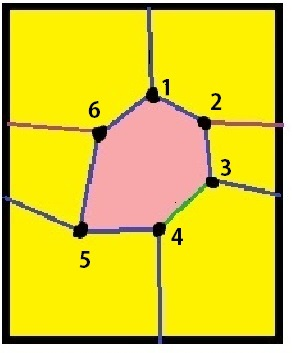
\includegraphics[scale=0.75]{packing_cartoon_edges.jpg}
\caption{  A primitive cartoon of a cell packing with periodic boundary conditions. Note that the edge connecting vertices 3 and 4 is colored green, to denote an edge that is not affected by the size of the periodic box. The edge connecting vertices 2 and 6 is colored purple, and denotes an edge that \ul{is} affected by the size of the periodic box.}
\label{fig:packing}
\end{center}
\end{figure}
For this edge, we have to consider the coordinates system of this box. I am treating the bottom left corner of this box as the origin $(0,0)$. The bottom edge of the box has the coordinate $y = 0$ and the left edge of the box has the coordinate $x = 0$. Then, the right edge of the box has an x- coordinate or $x = L_x$. Knowing this, we can find the length of the purple edge:
\begin{center}
\begin{equation}
l_j = \sqrt{(L_x - r_{2x} + r_{6x})^2 + (r_{2y} - r_{6y})^2}
\end{equation}
\end{center}
From this illustration, we can then see that only edges that cross over the edge are relevant for the derivative with respect to box size. Looking at the lengths of those edges, we can find our derivative nicely:
\begin{center}
\begin{equation}
\label{edgederivativebox}
\begin{split}
\pdv{L_x} (\sum\limits_{edges\hspace{1mm}crossing\hspace{1mm}L_x} l_j) &= \sum\limits_{edges\hspace{1mm}crossing\hspace{1mm}L_x} \cfrac{ \vb{l_j} \cdot {\vu{x}} }{l_j} = \sum\limits_{edges\hspace{1mm}crossing\hspace{1mm}L_x} \sin\theta_k\\
\pdv{L_y} (\sum\limits_{edges\hspace{1mm}crossing\hspace{1mm}L_y} l_k) &= \sum\limits_{edges\hspace{1mm}crossing\hspace{1mm}L_y} \cfrac{ \vb{l_k} \cdot {\vu{y}} }{l_k} = \sum\limits_{edges\hspace{1mm}crossing\hspace{1mm}L_x} \sin\theta_k\\
\end{split}
\end{equation}
\end{center}
Note that $\vb{l_j}$ or $\vb{l_k}$ are the vectors connecting the two vertices of edges $j$ and $k$ respectively. $\vu{x}$ and $\vu{y}$ are the unit vectors in the $x$ and $y$ direction respectively. $\theta_k$ is the angle the crossing edge makes with the wall of the box that was crossed. Ultimately, we can summarize Eqn. \ref{edgederivativebox} by saying that the derivative of the interfacial tension portion of the energy is proportional to the sine of the angle that the crossing edge makes with the box wall it crosses. This can also be written as proportional to the angle that the edge makes with either the x or y axis, depending on what is easier for the simulation. 

Note, what this tells us is that the derivative of the tension energy with respect to the box wall is the sum over the product of the tensions along each crossing edge times the ``direction sine" of each crossing edge with the respective box wall.
\subsubsection{$\frac{k}{2} \sum\limits_{cells\hspace{1mm}i} A_i^2$}
We can start with the chain rule to isolate the term we're looking for:
\begin{center}
\begin{equation}
\pdv{L_x} (\frac{k}{2} \sum\limits_{cells\hspace{1mm}i} A_i^2) =  k \sum\limits_{cells\hspace{1mm}i} A_i \pdv{A_i}{L_x}
\end{equation}
\end{center}
An analogous expression exists for $\pdv{L_y}$. Now we have to look for where the box size appears in the individual cell areas. Just like with the previous subsubsection, we can note that only the cells that cross over the box walls will be relevant to the calculation.

\begin{figure}[H]
\begin{center}
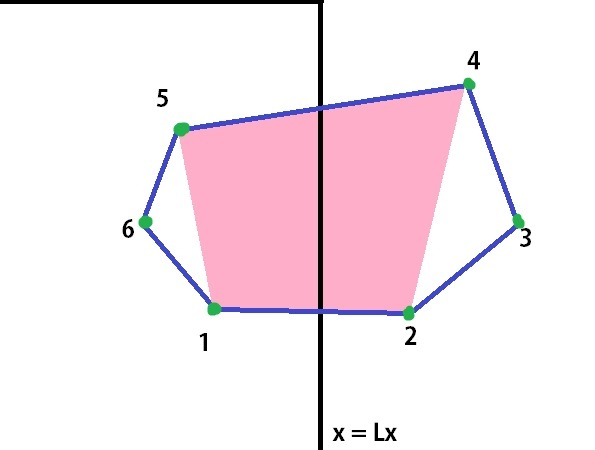
\includegraphics[scale=0.75]{packing_cartoon_areas_2.jpg}
\caption{  A primitive cartoon of a cell crossing the $x = L_x$ boundary, to help illustrate the calculation of $\pdv{A}{L_x}$.   The pink shaded region highlights the area relevant to the calculation of said derivative.}
\label{fig:cellareas}
\end{center}
\end{figure} 
Using \ref{fig:cellareas}, we can start calculating our derivative.
\begin{center}
\begin{equation}
\begin{split}
A = \sum\limits_{\text{vertices}} \frac{\vu{z}}{2} \cdot [\vb{r}_i \times \vb{r}_{i+1}]
\end{split}
\end{equation}
\end{center}
For the above equation, $i$ ranges from $1-6$ and back to $1$, (so for the purposes of the sum, $\vb{r}_{6+1} = \vb{r}_{1}$).  
\begin{center}
\begin{equation}
\begin{split}
A &= \frac{1}{2}[ (r_{1x} r_{2y} - r_{2x} r_{1y}) + (r_{2x} r_{3y} - r_{2y} r_{3x}) + (r_{3x} r_{4y} - r_{4x} r_{3y}) + ( r_{4x} r_{5y} - r_{5x} r_{4y}) + \\ &\hspace{3cm}(r_{5x} r_{6y} - r_{6x} r_{5y}) + (r_{6x} r_{1y} - r_{1x} r_{6y})]
\end{split}
\end{equation}
\end{center}
We can plug in some of these values that will include $L_x$:
\begin{center}
\begin{equation}
\begin{split}
A &= \frac{1}{2}\{ [(r'_{1x})  r_{2y} - (r'_{2x} + L_x) r_{1y}] + [(r'_{2x} + L_x) r_{3y} - (r'_{3x} + L_x) r_{2y}] + [(r'_{4x} + L_x) r_{5y}-\cdots \}
\end{split}
\end{equation}
\end{center}
Primed coordinates refer to coordinates that take periodic boundary conditions into account. So for example, $r_{2x} = r'_{2x} + L_x$. $r_2x$ would be the coordinates of vertex 2 without PBC where as $r'$ are the coordinates of vertex 2 in our simulation. The ellipses are the contributions to the area without any $L_x$'s. Now, we are ready to take the derivative:
\begin{center}
\begin{equation}
\begin{split}
\pdv{A}{L_x} &= \frac{1}{2} \{-r_{1y} - r_{3y} - r_{2y} + r_{4y} + r_{3y} + r_{5y} \}\\
 &= \frac{1}{2} \{[r_{5y} - r_{1y}] + [r_{4y} - r_{2y}] \}
\end{split}
\end{equation}
\end{center}
So this would the value for the derivative of the cell in Fig. \ref{fig:cellareas}. In general, we can interpret this derivative if we establish some new terminology for our vertices. In Fig. \ref{fig:cellareas}, we can identify vertices 1,2,4, and 5 as ``crossing edge vertices". Then the edges connecting vertices 1 and 2 and 4 and 5 are ``crossing edges." The derivative of the cell area with respect to $L_x$ is effectively the difference of the average y-coordinate of the edge-sharing crossing edge vertices (i.e. so vertex pairs 1 \& 2 and 4 \& 5 are ``edge-sharing crossing edge vertices"). With that in mind, here's a rough algorithm for finding this derivative:
\begin{enumerate}
\item Undo pbc
\item Identify crossing edges (maybe switch 1 and 2)
\item take average of y-coordinate between edge-sharing vertices
\item Find the difference
\end{enumerate}
For completeness, I can attempt to write out  meaningful equations the derivatives:
\begin{center}
\begin{equation}
\label{dadlx}
\pdv{A}{L_x} = \{ [\text{avg y-coordinate of upper crossing edge }] - [\text{avg y-coordinate of lower crossing edge}]\}
\end{equation}
\end{center}
and we can do another one for $\pdv{A}{L_y}$.
\begin{center}
\begin{equation}
\label{dadly}
\pdv{A}{L_y} = \{[\text{avg x-coordinate of right crossing edge}] - [\text{avg x-coordinate of left crossing edge}]\}
\end{equation}
\end{center}
\begin{comment}
This term is by far the most complicated one. We can start with some chain rule:
\begin{center}
\begin{equation}
\pdv{L_x} (k \sum\limits_{cells\hspace{1mm}i} A_i^2) = 2 k \sum\limits_{cells\hspace{1mm}i} A_i \pdv{A_i}{L_x}
\end{equation}
\end{center}
An analagous expression exists for $\pdv{L_y}$. Now, we have to look for where the box size appears in the individual cell areas. Just like with the previous subsubsection, we can note that only the cells that cross over the box walls will be relevant to the calculation. Noting this, we can identify a few relevant cases to study. 
\begin{figure}[H]
\begin{center}
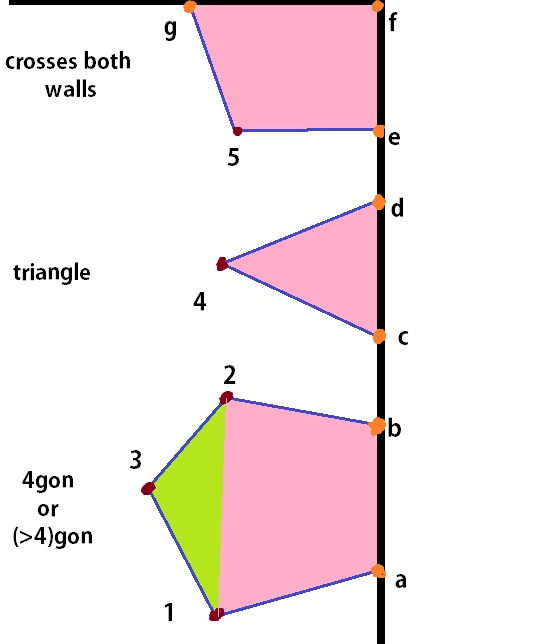
\includegraphics[scale=0.75]{packing_cartoon_areas.jpg}
\caption{  A primitive cartoon of the different types of geometries that cross over cell boundaries. The bottom case is effectively the most general and occurs when a cell crosses over a boundary and has more than 1 of its actual vertices showing. If we count that box wall, it makes a ``$4$gon" or a ``($>4$)gon" with the wall. The middle case shows a cell with only one of its real vertices left of the wall; this makes a triangle with the box wall. The final case at the top is for a cell that crosses both top and right walls. Here, only one vertex is showing. The pink regions highlight the portion of each cell that is relevant for the calculation of our derivative. Thus, if we removed the green section of the bottom example, it would not affect the shape's derivative with respect to the box size. Note that "actual" vertices, which denote the cells, are labeled with numbers and scarlet dots. The "fake" vertices, which are created by including the box walls as part of the cell shape, are labelled with letters and orange dots.  }

\label{fig:cellareas}
\end{center}
\end{figure}
I will only explicitly show the calculation for the bottom 5gon in Fig. \ref{fig:cellareas} and then argue why the other two cases shown are just special cases of that one. \\ \\
Begin by noting that we can use the shoelace formula to find the area of the entire cell. We can split this formula up into two areas: 
\begin{center}
\begin{equation}
A_i = A_i^{(left)} + A_i^{(right)}
\end{equation}
\end{center}, where $A_i^{(left)}$, the left area, is what we are shown and $A_i^{(right)}$, the right area, would be on the other side of the wall. Because of PBC, the right area is on the other side of the packing, and sees the wall it crosses as having x-coordinate $0$ intsead of $L_x$, we can ignore it. Then, we can rewrite the shoelace formula for the 5gon in Fig. \ref{fig:cellareas} as:
\begin{center}
\begin{equation}
\label{eqn: shoelace}
\begin{split}
A_i^{(left)} &= \sum\limits_{vertices \hspace{1mm} l} \frac{\vu{z}}{2} \cdot \big[ \vb{r_{il} } \times\vb{r_{i(l+1)}}\big]
\end{split}
\end{equation}
\end{center}
where the index $l$ cycles through indices $1, a, b, 2, 3,$ and back to $1$. The vectors $r_j$ represent the coordinates of the vertices of the 5gon. For the next parts of the calculation, I will drop the index i and the superscript ``left.":
\begin{center}
\begin{equation}
\begin{split}
A &= \frac{\vu{z}}{2} \cdot \big[(\vb{r}_1 \times \vb{r}_a) + (\vb{r}_a \times \vb{r}_b) + (\vb{r}_b \times \vb{r}_2) + (\vb{r}_2 \times \vb{r}_3) + (\vb{r}_3 \times \vb{r}_1)\big] \\
&= \frac{1}{2} [(r_{1x} r_{ay} - r_{1y} r_{ax})+ (r_{ax} r_{by} - r_{ay} r_{bx}) + ( r_{bx} r_{2y} - r_{by} r_{2x}) + (r_{2x} r_{3y} - r_{2y} r_{3x}) + \\ & \hspace{2cm} (r_{3x} r_{1y} - r_{3y} r_{1x})]\\ &= \frac{1}{2}[(r_{1x} r_{ay} - r_{1y} L_x)+ (L_x r_{by} - r_{ay} L_x) + ( L_x r_{2y} - r_{by} r_{2x}) + (r_{2x} r_{3y} - r_{2y} r_{3x})+ \\ & \hspace{2cm} (r_{3x} r_{1y} - r_{3y} r_{1x})]\\
\end{split}
\end{equation}
\end{center}
We are taking a derivative with respect to $L_x$, so we can drop all other terms and take our derivative:
\begin{center}
\begin{equation}
\pdv{A}{L_x} = \frac{1}{2} \big[r_{2y} - r_{1y} + r_{by} - r_{ay} \big]
\end{equation}
\end{center}
This formula is not very easy to generalize. Here, I will try to generalize the equation in order to explain why the other two examples in Fig. \ref{fig:cellareas} are just special cases.\\ \\
We can call vertices $a$ and $b$ wall vertices and note that every cell that crosses over the right boundary will have two wall vertices. For cells that cross two boundaries, like the upper most example in Fig. \ref{fig:cellareas}, the  corner of the box at coordinates is a wall vertex. For the upper most example cell in Fig. \ref{fig:cellareas}, I will NOT call vertex $g$ a wall vertex. Because it's not on the right wall of the box, the fact that it is on a wall is not why it would affect the final derivative of that 4gon's area with respect to $L_x$. Instead, will introduce the term "wall neighbor vertex" to describe vertices like $g$ or $5$ or even $1$ and $2$, which have as a neighbor at least one wall vertex. With these two terms, we can come up with a nice formula for our derivative:
\begin{center}
\begin{equation}
\label{dAdLx}
\pdv{A}{L_x} = \frac{1}{2} \bigg[|y_{\text{neighbor\hspace{1mm}1}} - y_{\text{neighbor\hspace{1mm}2}}| + |y_{\text{wall\hspace{1mm}1}} - y_{\text{wall\hspace{1mm}2}}| \bigg]
\end{equation}
\end{center}
Where $y_{\text{neighbor}}$ is the y-coordinate for the wall neighbor vertex and $y_{\text{wall}}$ is the y-coordinate for the wall vertex. The absolute value is included just so that the labelling or the different vertices does not affect the sign of the result (which should be positive, since I was careful to add up vertex products in a counterclockwise fashion, according to the right hand rule). This formula can be applied as is to the bottom 5gon in Fig \ref{fig:cellareas}. To apply this to the 4gon that crosses both boundaries, one needs to keep in mind that vertex $g$ need be considered a neighbor vertex, since it does not have an x-coordinate $L_x$. For the triangle (or 3gon, for consistency) in the figure, note that the two wall vertices just have the same neighbor vertex. Thus, the term that denotes the difference in the y-coordinates of the neighbor vertex is $0$ for triangles. We can nicely right this formula for $\pdv{A}{L_y}$:
\begin{center}
\begin{equation}
\label{dAdLy}
\pdv{A}{L_y} = \frac{1}{2}\bigg[|x_{\text{neighbor\hspace{1mm}1}} - x_{\text{neighbor\hspace{1mm}2}}| + |x_{\text{wall\hspace{1mm}1}} - x_{\text{wall\hspace{1mm}2}}| \bigg]
\end{equation}
\end{center}
Of course, we should note that Eqns \ref{dAdLx} and \ref{dAdLy} are only non-zero for cells crossing the right and upper box walls respectively. \\ \\
To sanity check this calculation, I wanted to confirm that $\pdv{L_x} \sum A_i = \sum \pdv{A_i}{L_x} = L_y$. I could not find any means to do this calculation in general, but I can confirm for the sample packing for which I did this calculation that it works. The general explanation is as follows: In a confluent packing, neighboring cells that cross the boundary share wall vertex and wall neighbor vertex pairs. However, because of the handedness of the equations, they will have opposite signs in the derivatives of different cell areas. Thus, when we sum of the derivatives of all the crossing cells, every term cancels except for the coordinates of the top wall/neighbor vertex pair and the bottom wall/neighbor vertex pair. The top wall/neighbor pair have y-coordinates $L_y$ and the bottom wall/neighbor pair have y-coordinates $0$. Thus, the result of the sum is $\frac{1}{2} (2 L_y) = L_y$. For anyone who wishes to calculate this and convince themselves of this, here is a sample packing that I used:
\begin{figure}[H]
\begin{center}
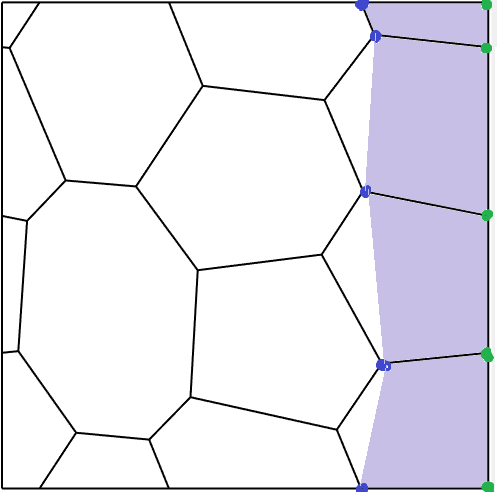
\includegraphics[scale=0.70]{frame_009.png}
\caption{ A sample confluent packing which I used to sanity check my formalism for the derivative of cell areas with respect to the box size. Wall (green) and neighbor (blue) vertices as well as relevant areas (purple-grey) are marked for convenience.}
\label{fig:samplepacking}
\end{center}
\end{figure}
\end{comment}
\section{Full Dynamics}
Now, we finally have all the essential dynamics for an NPT vertex model ensemble. Here's the list of equations:
\begin{center}
\begin{equation}
\label{eqn: coordinatedyn}
\pdv{\tilde{x_i^n}}{t} = -\nu \pdv{E_0}{\tilde{x_i^n}} \rightarrow \pdv{x_i^n}{t}  = -\nu |L_i(t)|^2\pdv{E_0}{x_i^n} + \frac{x_i^n}{F_{ii}} \pdv{F_{ii}}{t}
\end{equation}
\end{center}
We can pick either set of equations for the dynamics of the coordinates. For the unscaled coordinates, we need the deformation gradient dynamics:
\begin{center}
\begin{equation}
\label{eqn: deformationdyn}
\pdv{F_{\beta \beta}}{t} = -\mu\bigg\{\sum\limits_{n} \pdv{E_0}{x_\beta^n}  \cfrac{x_\beta^n}{F_{\beta \beta}} +  \pdv{E_0}{|\vb{L}_\beta|} L_{\beta \beta} + p \cfrac{A(t)}{F_{\beta\beta}}\bigg\}
\end{equation}
\end{center}
This equation basically says that the dynamics of the deformation gradient are linear in an external pressure minus an interior pressure. The $\pdv{E_0}{|\vb{L}_\zeta|}$ term is left as is because writing out its full form deserves a line of its own.
\begin{center}
\begin{equation}
\label{eqn: pbcd}
\pdv{E_0}{|\vb{L}_\zeta|} = k \bigg( \sum\limits_{\text{cells i}} A_i \pdv{A_i}{|\vb{L}_\zeta|} - A_0 |\vb{L}_\eta| |\epsilon_{\zeta \eta}|\bigg) + \gamma \sum\limits_{\text{EC}\zeta\text{ k}} \cos(\vb{l}_k, \vu*{\zeta}) 
\end{equation}
\end{center}
Lots to explain here. $\zeta$ runs over the two different coordinate axes. $L_\eta \epsilon_{\zeta\eta}$ uses the 2D Levi-Cevita tensor to denote that if the derivative is with respect to $x$, $\eta = y$ and vice versa. The absolute value on the Levi-Cevita tensor are necessary because it's an anti-symmetric tensor and we do not want the negative sign in this formula whether or not the permutation of indices is odd. The index label ``ECX" stands for "edges crossing the right boundary. ``ECY" stands for ``edges crossing the upper boundary." In the sum above, I use $``EC{\zeta}"$ as a stand-in for the two. I switched up the formalism for the edge derivatives by introducing direction cosine notations. Thus, $\cos(\vb{l}_m, \vu{y})$ is effectively the cosine of the angle between edge $\vb{l}_m$ and the unit vector in the y direction. Once again, we have another derivative that deserves its own subsubsection that I won't explicitly write out as part of this larger formula. For $\pdv{A_i}{{\vb{L}_\zeta}}$, I refer readers to Eqns \ref{dadlx} and \ref{dadly}.Also, if we let each cell have its own preferred area, we would instead write:
\begin{center}
\begin{equation}
\label{eqn: pbcd2}
\pdv{E_0}{|\vb{L}_\zeta|} = k \sum\limits_{\text{cells i}} (A_i - A_0) \pdv{A_i}{|\vb{L}_\zeta|} + \gamma \sum\limits_{\text{EC}\zeta\text{ k}} \cos(\vb{l}_k, \vu*{\zeta}) 
\end{equation}
\end{center}
\section{Internal Stress Tensor}

One of the expectations for the dynamics of the box size is that they roughly depend on an internal stress minus an external pressure. Using Doi and Edwards (The Theory of Polymer Dynamics), we can verify this. From section 3.7.4 of the text, we expect the internal stress to look like:
\begin{center}
\begin{equation}
\label{eqn: doiedwards_internalstress}
\sigma_{\alpha \beta} = -\frac{1}{A} \sum\limits_{\text{particles m}} \expval{F_\alpha^m R_\beta^m}
\end{equation}
\end{center}
Here, the average refers to the configurational average of the "beads" (objects undergoing Brownian motion in the fluid). Thus, the average would be calculated by integrating with probability distribution $\Psi$, the solution to the Smoluchowski equation. However, since we are doing our dynamics at $T=0$, our $\Psi$ is a delta function and we can effectively drop the angle brackets. $F_\alpha^m$ refers to the $\alpha$-component of the force on particle or bead $m$. $R_\beta^m$ is the $\beta$-coordinate of the position of particle $m$. \\ \\
To compare this against the above calculations, we can write this in a nicer form:
\begin{center}
\begin{equation}
\label{eqn: stress_alternative}
\sigma_{\alpha \beta} = \frac{1}{A} \sum\limits_{\text{particles m}} \pdv{U}{R_\alpha^m} R_\beta^m
\end{equation}
\end{center} 
Which is beginning to resemble Eqn \ref{eqn: deformationdyn}. What we can recognize to match the two is that the stress is effectively the sum of the outer products between degrees of freedom of the system and the derivative of the energy with respect to said degrees of freedom. This means a slight tweak of the notation:
\begin{center}
\begin{equation}
\label{eqn: dof}
\sigma_{\alpha \beta} = \frac{1}{A} \sum\limits_{\text{d.o.f m}} \pdv{U}{q_\alpha^m} q_\beta^m
\end{equation}
\end{center}
where we borrow "q" from the notation of generalized coordinates to show that not all the degrees of freedom need to be positions. Now that we have added the box walls as degrees of freedom, this important to note for this calculation. In our case, we can note that:
\begin{center}
\begin{equation}
\label{eqn: absc}
\pdv{U}{q_\alpha^m} q_\beta^m = \sum\limits_{\text{coordinates}}\pdv{U}{R_\beta^m} R_\alpha^m + \sum\limits_{\text{box walls}}\pdv{U}{L_\alpha^m} L_\beta^m
\end{equation}
\end{center}
which we can recognize as part of Eqn \ref{eqn: deformationdyn}. In fact, we can rewrite that equation in terms of external stress and external stress:
\begin{center}
\begin{equation}
\label{eqn: deformationdyn2}
\begin{split}
\pdv{F_{\beta \beta}}{t} & = -\mu\bigg\{\sum\limits_{n} \pdv{E_0}{x_\beta^n}  \cfrac{x_\beta^n}{F_{\beta \beta}} + \pdv{E_0}{|\vb{L}_\beta|} L_{\beta \beta} + p \cfrac{A(t)}{F_{\beta\beta}}\bigg\}\\
&= -\mu\bigg\{\sum\limits_{n} \pdv{E_0}{x_\beta^n}  \cfrac{x_\beta^n}{F_{\beta \beta}} +  \pdv{E_0}{|\vb{L}_\beta|} \frac{|\vb{L}_{\beta}|}{F_{\beta\beta}} + p \cfrac{A(t)}{F_{\beta\beta}}\bigg\}\\
&= -\mu\bigg\{\frac{\sigma_{\beta \beta} A(t)}{F_{\beta \beta}} + \frac{p A(t)}{F_{\beta \beta}}  \bigg\}\\
&= -\frac{\mu A(t)}{F_{\beta \beta}} (\sigma_{\beta\beta} + p).
\end{split}
\end{equation}
\end{center}
\section{Purpose of Box Length Derivative}
In the dynamics of the box, it is not immediately clear what the purpose of the $\pdv{E}{|\vb{L}|}$. However, it appears that this term has been well studied in the literature of periodic boundary conditions in both MD and Langevin dynamics simulations. Ultimately, many of the papers (which I will mention here) that discuss this point turn to the virial theorem to demonstrate this. \\ \\
One of the ways to write the virial theorem for atoms with some potential $U$ is in terms of pressure:
\begin{center}
\begin{equation}
\label{eqn: virial}
p = -\expval{\pdv{E}{V}} = -\expval{\pdv{T}{V}} - \expval{\pdv{U}{V}} = \frac{N k_B T}{V} - \frac{1}{3 V} \expval{\sum\limits_i r_i \pdv{U}{r_i}}
\end{equation}
\end{center} 
where we take advantage of the fact that:
\begin{center}
\begin{equation}
\label{eqn: dudv}
\pdv{U}{V} = \frac{1}{3 V} \sum\limits_i r_i \pdv{U}{r_i}
\end{equation}
\end{center}
for particles with an interacting potential. However, as is well documented in several of these papers, this theorem has to change for cases of periodic boundary conditions. Taken from Louwerse et al (who assume a cubic periodic box), we can see this derivation:
\begin{center}
\begin{equation}
\begin{split}
\dv{U}{V} &= \dv{L}{V} \bigg(\pdv{U}{L} +\sum_{i=1}^{N}\dv{\vb{r}_i}{L} \cdot \pdv{U}{\vb{r}_i} \bigg)\\
&= \frac{1}{3 L^2} \bigg(\pdv{U}{L} +\sum_{i=1}^{N}\frac{\vb{r}_i}{L} \cdot \pdv{U}{\vb{r}_i}\bigg)\\
&= \frac{1}{3V} \sum_{i=1}^{N}\frac{\vb{r}_i}{L} \cdot \pdv{U}{\vb{r}_i} + \frac{1}{3 L^2} \pdv{U}{L}
\end{split}
\end{equation}
\end{center}
which would change the virial theorem to something like:
\begin{center}
\begin{equation}
\label{eqn: virialedit}
p = \frac{N k_B T}{V} - \expval{\frac{1}{3V} \sum_{i=1}^{N}\frac{\vb{r}_i}{L} \cdot \pdv{U}{\vb{r}_i} + \frac{1}{3 L^2} \pdv{U}{L}}
\end{equation}
\end{center}
Perhaps it wasn't necessary to show the full derivation, but ultimately, the derivative of a periodic potential with respect to the volume resulted in a necessary $\pdv{U}{L}$ term. Physically, this implies that when the particle coordinates are fixed, changing the volume of the periodic box can change the potential. This makes sense; after all, if you hold the position of the particles fixed and increase the size of the box, you're increasing the distance between particles in the box and the periodic copies of those particles in neighboring "boxes." Likewise, in our case, if we were to increase box size while holding vertices fixed, we would change the orientation and length of the boundary crossing edges, which would in turn change the areas of the cells crossing the boundary. This change that is necessary for the virial theorem applies to any equation that uses a derivative of the periodic potential with respect to volume or a deformation gradient component. 
\subsection{Papers that mention this}
Louwerse, Manuel J. Baerends, Evert Jan. (2006). ``Calculation of pressure in case of periodic boundary conditions".\textit{ Chemical Physics Letters}.  \\ \\ 
Swenson, Robert J. (1982). ``Comments on virial theorems for bounded systems." \textit{American Journal of Physics}. \\ \\
D. Tsai, ``The virial theorem and stress calculation in molecular dynamics,”
The Journal of Chemical Physics, vol. 70, no. 3, pp. 1375–1382, 1979. 
\\ \\	
\subsection{Simple Model Calculation}
Here, I try some simple calculations to show the role of the length derivative. I try two models here. The first is a 1D model where I ignore external pressure. 
\begin{figure}[H]
\begin{center}
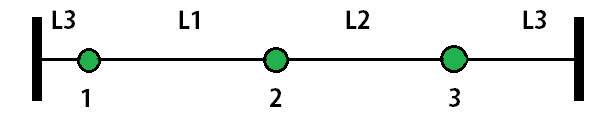
\includegraphics[scale=1.0]{1D_toy_sample_model.png}
\caption{1D Vertex model. In practice, this is just a line of vertices. The ``box" length is $L_1 + L_2 + L_3 = L$. Here, the labels ``L1" labels the edges and not the length of the edges, which is why there are two L3's.}
\label{1dvertexmodel}
\end{center}
\end{figure}

We can analyze the dynamics of this model. So assuming periodic boundary conditions, we can say:
\begin{center}
\begin{equation}
E = \gamma (L_1 + L_2 + L_3) = \gamma [(x_2-x_1)+(x_3-x_2)+(x_1+L-x_3)] = \gamma L
\end{equation}
\end{center}
As a result, the energy is not a function of the vertex positions. As a result, the scaled coordinates do not change over the course of the simulation. However, the deformation gradient does change.
\begin{center}
\begin{equation}
\dv{F}{t} = -\mu\bigg[\pdv{E}{F}\bigg] = -\mu\bigg[\pdv{E}{L}\bigg\vert_{x} \pdv{L}{F}\bigg] = -\mu\big[\gamma L_0\big].
\end{equation}
\end{center}
The $L_0$ is the initial length of the ``packing". There is only one term in the above calculation because $\pdv{E}{x_i} = 0$ for any vertex $i$ in this system. Thus, in this simple model, the derivative with respect to the length is responsible for the model behaving correctly. After all, with constant tensile forces on all the vertices, we expect this packing to constantly decrease in size and minimize the overall energy. We can also speculate that this term gives us the ability to place the box boundaries anywhere on the periodic system and get the same dynamics. However, it seems easier to see this in a slightly more complicated model. 
\begin{figure}[H]
\begin{center}
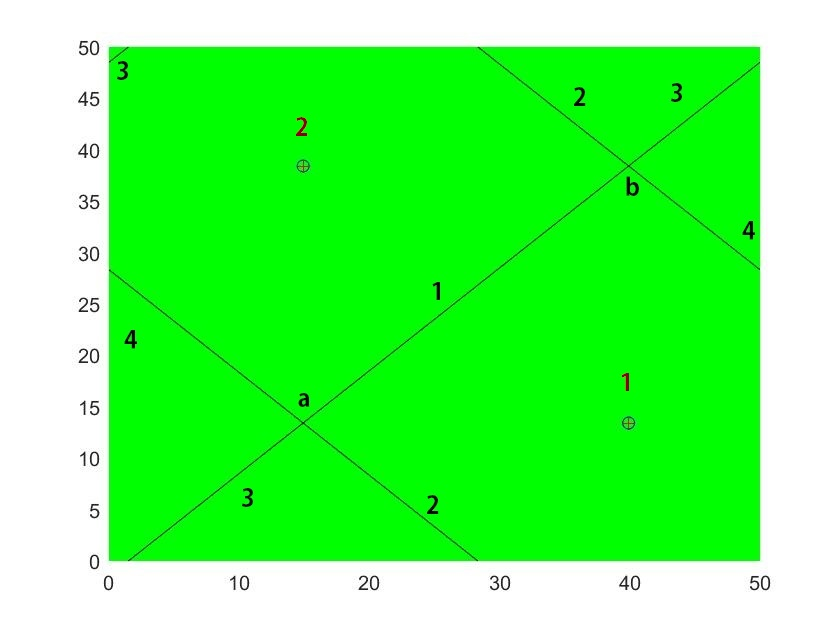
\includegraphics[scale=0.6]{simplest_vertex_model.jpg}
\caption{Simplified 2D vertex model. This packing has two cells and has been equilibrated. Edges are labelled with numbers and vertices are labelled with letters. The centroid of each of the cells is marked with a red cross and a magenta number above it. These numbers label the cells as cell 1 and cell 2. }
\label{simple2dmodel}
\end{center}
\end{figure}
\begin{figure}[H]
\begin{center}
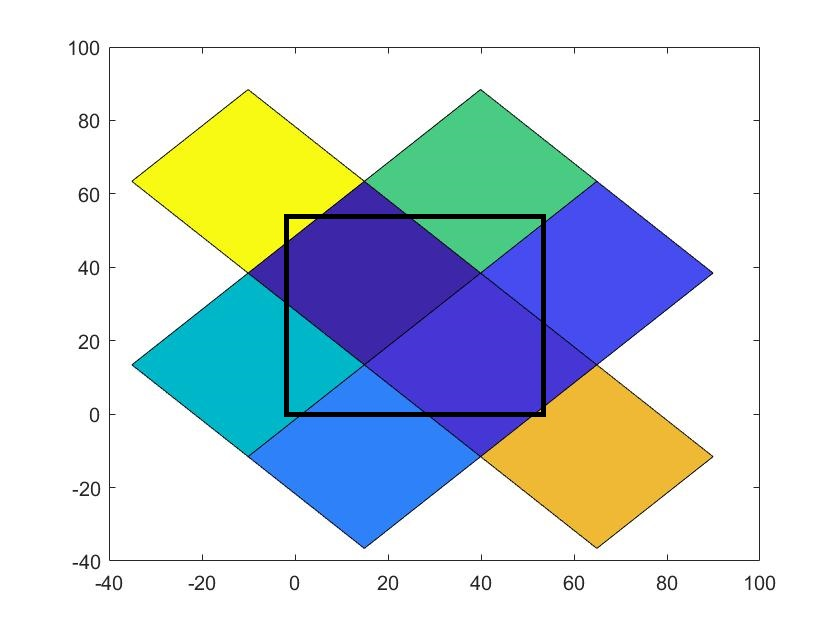
\includegraphics[scale=0.6]{periodicpacking_simplest_vertex_model_window.jpg}
\caption{A section of the periodic packing generated in MATLAB with a window superimposed to show the section represented in Fig \ref{simple2dmodel}. Unfortunately, I wasn't able to put in a fuller representation of the infinite packing, but with some imagination, you can see that moving the window around would result in the exact same number of edges and vertices. Additionally, the exact same areas of each of the cells would be captured in the window (this is a trivial fact). However, playing with this window and doing this thought experiment leads me to believe that the derivative with respect to length remains constant no matter how the window is selected (potentially also trivial).}
\end{center}
\end{figure}

For the above 2D packing, I'm going to make some simplifying assumptions. First, I am going to claim that the packing is equilibrated such that all the cell areas are the preferred area and the tension forces are perfectly balanced. This implies that $\pdv{E}{\tilde{x}} = 0$. Then, we can look at the dynamics of the deformation gradient (just the $F_{xx}$ term):
\begin{center}
\begin{equation}
\dv{F_{11}}{t} = -\mu\bigg[\pdv{E}{L_1}\bigg\vert_{\vb{x}} L_{11}\bigg] = 2\gamma \cos(\vu{x}, \vu{l}_3)
\end{equation}
\end{center}
So in this case, the only forces acting on the box are the tension forces of the two edges crossing over the right boundary. As we move the window across the packing, no matter what, two edges will cross the box boundary at the same angle. \\ \\
To gain  a bit more insight, let's perturb one of the vertices, such that we do not have a force balance about each vertex and the areas are perturbed away from the preferred area. The vertices will now have non-zero dynamics of course, but I want to only focus on the deformation gradient dynamics. The above equation becomes:
\begin{center}
\begin{equation}
\label{eqn: f11_checks}
\dv{F_{11}}{t} = -\mu\bigg[\pdv{E}{x_1^1}\frac{x_1^1}{F_{11}} + \pdv{E}{x_1^2}\frac{x_1^2}{F_{11}} + \pdv{E}{L_1} L_{11} \bigg]
\end{equation}
\end{center}
The last term can be calculated pretty simply:
\begin{center}
\begin{equation}
\pdv{E}{L_1} = \gamma \bigg( \cos(\vu{x}, \vu{l}_3) + \cos(\vu{x}, \vu{l}_4)\bigg) + \frac{k L_y}{2} \bigg[ (A_1 - A_0) + (A_2 - A_0)\bigg]
\end{equation}
\end{center}
The area terms here are simpler to calculate than normal because there are so few cells and the areas relevant to the calculation (think of the pink region in Fig \ref{fig:cellareas}) are triangles. The reason I wanted to continue this thought experiment with a perturbation is to test whether this derivative correct for changes in the box location. Looking at the above expression, it is not hard to convince oneself that this expression is independent of box location (as we expect it to be, since a derivative of energy should be independent of location). It is also possible to see that any perturbations to the box location do not affect the first two terms in Eqn. \ref{eqn: f11_checks} (because of Newton's Third Law). \\ \\
Based on this analysis, it seems like the forces that appear to act on the boundary are the result of periodic boundary conditions. The forces acting on the tissue from the other side of the wall (wrap-around forces due to pbc) appear in the derivative of the energy with respect to length. It appears that even when the net forces on all the vertices are $0$, there can still be forces on the walls. It appears that this is because of the local forces at the boundary of the tissue that are not equilibrated (the way the forces int the center of the tissue are). 


\section{Implementing this Formalism}

To minimize the changes that need to be made to the code, I want to adapt this formalism as much as I can to Meryl's original notation. Here, I will record these adaptations.

\subsection{Mobility Terms}
The simplest change to make was in the mobility terms. I use $\nu$ for the mobility of the scaled coordinates and $\mu$ for the mobility of the box walls in this document. Meryl uses $\alpha_M$ as the friction of the unscaled coordinates and $\alpha_T$ as the friction of the box walls. As a consequence of this, I need to reassign $\nu = \frac{1}{\alpha_M}$ and $\mu = \frac{1}{\alpha_T}$ in my dynamics when implementing them into the vertex model. 
\subsection{Avoiding Deformation Gradient}
The above formalism uses a deformation gradient to allow the box to change while maintaining constant pressure. Currently, only external hydrostatic pressure is allowed for (see Eqn.  \ref{eqn: boxenergy}). This energy will have to change in the future if we are interested independent constant external stresses on each of the box dimensions. \\ \\
But more to the point, if I were to implement the equations derived in this document verbatim, I would have to change all of Hayden's integrator code and make sure the dynamics of the deformation gradient are accounted for. I have found that this can be sidestepped by simply reintroducing the length of the box as the dynamical variable and including factors of $L_{xx}$ and $L_{yy}$. The dynamical equations for the system can be written, in the formalism of this document, as:

\begin{center}
\begin{equation}
\label{eqn: Fdyn}
\pdv{F_{\alpha\alpha}}{t} = -\mu \frac{A(t)}{F_{\alpha\alpha}} (\sigma_{\alpha\alpha} + p)
\end{equation}
\end{center}

$\sigma_{\alpha\alpha}$ refers to the ``$\alpha\alpha$" component of the internal stress tensor. For the code, we convert to dynamics of box length:
\begin{center}
\begin{equation}
\begin{split}
\pdv{F_{\alpha \alpha}}{t} L_{\alpha \alpha} &= -\mu \cfrac{A(t)}{\frac{L_\alpha}{L_{\alpha\alpha}}} L_{\alpha\alpha}(\sigma_{\alpha \alpha} + p) \\
\pdv{L_\alpha}{t} &= -\mu \frac{A(t)}{L_\alpha} L_{\alpha\alpha}^2 (\sigma_{\alpha\alpha} + p)
\end{split}
\end{equation}
\end{center}
which should lead to vertex dynamics that look like:
\begin{center}
\begin{equation}
\label{eqn: xdyn}
\pdv{x_i^n}{t} = -\nu L_i^2 \pdv{E_0}{x_i^n} - \frac{x_i^n}{L_i} \bigg[\mu \frac{A(t)}{L_i} L_{ii}^2(p + \sigma_{ii})\bigg]
\end{equation}
\end{center}
which means the final dynamics look like:
\begin{center}
\begin{equation}
\label{eqn: fullimplementdyn}
\begin{split}
\dot{L}_x &= -\frac{1}{\alpha_T} L_{xx}^2 L_y (\sigma_{xx} + p)\\
\dot{L}_y &= -\frac{1}{\alpha_T} L_{yy}^2 L_x (\sigma_{yy} + p)\\
\dot{x}^n &= -\frac{1}{\alpha_M} L_x^2 \pdv{E_0}{x^n} - \frac{1}{\alpha_T}\frac{x^n}{L_x} \bigg[ L_{xx}^2 L_y (p + \sigma_{xx})\bigg]\\
\dot{y}^n &= -\frac{1}{\alpha_M} L_y^2 \pdv{E_0}{y^n} - \frac{1}{\alpha_T}\frac{y^n}{L_y} \bigg[ L_{yy}^2 L_x (p + \sigma_{yy})\bigg]\\
\end{split}
\end{equation}
\end{center}

With these adjustments, the only major change to the dynamics has to be made in the ``ForceFunction," found in the the AGTissue class (AG = anisotropic growth). The numerical integrators can be left alone. 

\section{Length Dependent Drag }
The $L^2$ scaling in all the dynamics falls out naturally from the dynamical equations we began with. However, these give the simulation a characteristic timescale that varies with the size of the box. In practice (as of 6/3/20), the simulation also does not seem to be able to handle this scaling - the box becomes too big too fast and the vertex positions move unphysically). To handle this, we can look for ways to give length (or actually length squared) dependence to $\alpha_T$ and $\alpha_M$. The main constraint to do this will be the condition that we continue to satisfy the fluctuation dissipation theorem as we do this. Here, I will discuss some ideas I have as to how to do this.

\subsection{Multiplicative Noise in Scaled Coordinates}
The ultimate goal is to get a dynamical system that satisfies a Boltzmann distribution. Doi and Edwards gives us the theory for this. \\ \\
Without coordinate dependent drag, we know that the Smoluchowski equation is has a steady-state solution of a Boltzmann equation. However, with multiplicative noise, we need to add a new term to the Langevin equation so that it corresponds to a differential equation with a Boltzmann equation as its steady-state differential equation. 
\begin{center}
\begin{equation}
\label{eqn: Langevin eqn with extra term}
\dv{x_n}{t} = \sum\limits_m L_{nm} \bigg(-\pdv{U}{x_m} + f_m(t)\bigg) + \frac{1}{2} k_B T \sum\limits_{m} \pdv{x_m} L_{nm}
\end{equation}
\end{center}
The divergence of $L_{nm}$ is the extra term. $L_{nm}$ is the mobility matrix (contains inverse drag coefficients), $f_m$ is the random force, and $U$ is the potential. Here, the random noise has the following properties:
\begin{center}
\begin{equation}
\expval{f_m(t)} = 0, \hspace{1cm} \expval{f_m(t) f_n(t')} = 2 L_{nm}^{-1} k_B T \delta(t-t') \delta_{mn}
\end{equation}
\end{center}
Comparing this with our system of equations (in scaled coordinates):
\begin{center}
\begin{equation}
\label{eqn: sysofeqns}
\tilde{x}_i^n = -\frac{1}{\alpha_M^{i}} \pdv{H}{\tilde{x}_i^n} + B_n^i \eta_i^n(t), \hspace{1cm} F_{ii} = -\frac{1}{\alpha_T^i} \pdv{H}{F_{ii}} + C_{ii} \zeta_{ii}(t)
\end{equation}
\end{center} 
The noise terms ($\eta$ and $\zeta$) are Gaussian (see beginning of document for properties). The $\alpha$'s will contain coordinate dependent drag and so we will need to add an extra term to these eqns. $B_n^i = \frac{2 k_B T}{\alpha_M^i}$ and $C_n^i = \frac{2 k_B T}{\alpha_T^i}$. These make up the elements of our mobility matrix, which is diagonal in this case. Written out:
\begin{center}
\begin{equation}
\label{eqn: lmn}
L = \mqty(\dmat{\frac{1}{\alpha_M^x}, \frac{1}{\alpha_M^y}, \ddots, \frac{1}{\alpha_T^x}, \frac{1}{\alpha_T^y}})
\end{equation}
\end{center}
Now, we can look at Eqns \ref{eqn: fullimplementdyn} to see how to set $\alpha_M$'s and $\alpha_T$'s. Here's a proposed set:
\begin{center}
\begin{equation}
\alpha_M^x = \alpha_M^' L_{x}^2, \hspace{1cm}  \alpha_M^y = \alpha_M^' L_{y}^2, \hspace{1cm} \alpha_T^x = \alpha_T^' \cfrac{L_{xx}^2 L_{y}}{L_x}, \hspace{1cm} \alpha_T^y = \alpha_T^' \cfrac{L_{yy}^2 L_{x}}{L_y}
\end{equation}
\end{center}
This cancels out terms that change the characteristic timescale of the system. It also makes the box size proportional in box size ($\dot{L}_x \propto L_x$) which makes sense. Then, to guarantee a steady-state Boltzmann distribution, we can add the extra term to the Langevin equation:
\begin{center}
\begin{equation}
\begin{split}
\dv{t} \tilde{x}^n &= -\frac{1}{\alpha_M^x} \pdv{H}{\tilde{x}^n} + B_x^n \eta_x^n(t)\\  
\dv{t} \tilde{y}^n &= -\frac{1}{\alpha_M^t}\pdv{H}{\tilde{y}^n} + B_y^n \eta_y^n(t)\\
\dv{t} F_{xx} &= -\frac{1}{\alpha_T^x}\pdv{H}{F_{xx}} + C_{xx} \zeta_{xx}(t) + \frac{k_B T}{2 \alpha_T' L_{xx}^2 L_y}\\
\dv{t} F_{yy} &= -\frac{1}{\alpha_T^y} \pdv{H}{F_{yy}} + C_{yy} \zeta_{yy}(t) + \frac{k_B T}{2 \alpha_T' L_{yy}^2 L_x} \\
\end{split}
\end{equation}
\end{center}
This equations give us a Boltzmann distribution in scaled coordinates. 
\subsection{Proving that there exists a Boltzmann Distribution in (x,L) phase space}
For dynamical equations, we want to be sure that the probability of observing a given state in $({x}, {L})$ phase space is Boltzmann distributed. Carolina Baruffi's paper (see section 1) shows that this is the case for $({\tilde{x}}, {F})$ space. I'll extend this to the $({x}, {L})$ space. In the long time limit, the equilibrium probability distribution in scaled coordinate space is:
\begin{center}
\begin{equation}
\tilde{P}(\{\tilde{x}, F\}) = \tilde{Z}^{-1} \exp\bigg[\frac{\tilde{H}(\{\tilde{x}, F\})}{k_B T}\bigg]
\end{equation}
\end{center}
where the normalization constant is:
\begin{center}
\begin{equation}
\tilde{Z} = \int \exp\bigg[\frac{\tilde{H}(\{\tilde{x}, F\})}{k_B T}\bigg]\prod\limits_{n=1}^N \prod\limits_{i=1}^{2} \prod\limits_{j=1}^{2} d\tilde{x}_i^n dF_{jj}
\end{equation}
\end{center}
Our $\tilde{H}$ will not be the same as $\bar{H}$ used at the beginning of this document. The $\tilde{H}$ will be determined once we understand how the phase space volume element transforms. We transform the phase space volume element in the standard way (determinant of the a Jacobian):
\begin{center}
\begin{equation}
\label{eqn: phasespacetransform}
\prod\limits_{n=1}^N \prod\limits_{i=1}^{2} \prod\limits_{j=1}^{2} d\tilde{x}_i^n dF_{jj} = \frac{1}{A^N A_0}\prod\limits_{n=1}^N \prod\limits_{i=1}^{2} \prod\limits_{j=1}^{2} dx_i^n dL_j 
\end{equation}
\end{center}
Recall that $A_0 = L_{xx} L_{yy}$ and $A = A_0 \det F$. Now, we want a Boltzmann distribution in (x,L) space. We then expect the following to hold:
\begin{center}
\begin{equation}
\label{eqn: integrand}
\tilde{P}(\{\tilde{x}, F\}) \prod\limits_{n=1}^N \prod\limits_{i=1}^{2} \prod\limits_{j=1}^{2} d\tilde{x}_i^n dF_{jj} =  P(\{x,L\}) \prod\limits_{n=1}^N \prod\limits_{i=1}^{2} \prod\limits_{j=1}^{2} dx_i^n dL_j
\end{equation}
\end{center}
We can substitute Eqn \ref{eqn: phasespacetransform} into Eqn \ref{eqn: integrand}.
\begin{center}
\begin{equation}
\tilde{P}(\{x, F\}) \prod\limits_{n=1}^N \prod\limits_{i=1}^{2} \prod\limits_{j=1}^{2} d\tilde{x}_i^n dF_{jj} = P(\{x,L\}) (A^N A_0) \prod\limits_{n=1}^N \prod\limits_{i=1}^{2} \prod\limits_{j=1}^{2} d\tilde{x}_i^n dF_{jj}
\end{equation}
\end{center}
Then, we can say:
\begin{center}
\begin{equation}
P({x,L}) = \tilde{Z}^{-1} \exp\bigg[-\frac{\tilde{H}(\{\tilde{x}, F\})}{k_B T}\bigg] (A^{-N} A_0^{-1}) = \tilde{Z}^{-1} \exp\bigg[-\frac{\tilde{H}(\{\tilde{x}, F\})}{k_B T} - N \log A - \log A_0\bigg]
\end{equation}
\end{center}
Then, to make this a Boltzmann distribution, we know that
\begin{center}
\begin{equation}
\tilde{H} = \bar{H} - N k_B T \log A - k_B T \log A_0 = E_0 - pA - N k_B T \log A - k_B T \log A_0
\end{equation}
\end{center}
Then, with the above Hamiltonian, we can see that we do have a Boltzmann distribution in $x$ and $L$ phase space, even if we avoided solving a Stratonovich Fokker-Planck equation to find it. We can use this to correctly write down the dynamics of our system in $(\tilde{x}, F)$ phase space:
\begin{center}
\begin{equation}
\label{eqn: dyn}
\begin{split}
\dv{t} \tilde{x}^n &= -\frac{1}{\alpha_M^x} \pdv{\tilde{H}}{\tilde{x}^n} + B_x^n \eta_x^n(t)\\  
\dv{t} \tilde{y}^n &= -\frac{1}{\alpha_M^y}\pdv{\tilde{H}}{\tilde{y}^n} + B_y^n \eta_y^n(t)\\
\dv{t} F_{xx} &= -\frac{1}{\alpha_T^x}\pdv{\tilde{H}}{F_{xx}} + C_{xx} \zeta_{xx}(t) + \frac{k_B T}{2 \alpha_T' L_{xx}^2 L_y}\\
\dv{t} F_{yy} &= -\frac{1}{\alpha_T^y} \pdv{\tilde{H}}{F_{yy}} + C_{yy} \zeta_{yy}(t) + \frac{k_B T}{2 \alpha_T' L_{yy}^2 L_x} \\
\end{split}
\end{equation}
\end{center}
More details for the stochastic variables:
\begin{center}
\begin{equation}
\begin{split}
\expval{\eta_i^n} &= 0\\
\expval{\zeta_{\alpha\alpha}} &= 0\\
\expval{\eta_i^n(t) \eta_j^m(t') } &= \delta_{nm} \delta_{ij} \delta(t-t')\\
\expval{\zeta_{\alpha\alpha}(t) \zeta_{\beta\beta}(t')} &= \delta_{\alpha\beta} \delta(t-t')\\
\expval{\eta_i^n(t) \zeta_{\alpha\alpha}(t')} &= 0\\
\end{split}
\end{equation}
\end{center}
\section{Putting this all together}
So plugging in our drag terms (and dropping the primes):
\begin{center}
\begin{equation}
\label{eqn: fullimplementdyn}
\begin{split}
\dot{L}_x &= -\frac{1}{\alpha_T} L_{x} (\sigma_{xx} + p)\\
\dot{L}_y &= -\frac{1}{\alpha_T} L_{y} (\sigma_{yy} + p)\\
\dot{x}^n &= -\frac{1}{\alpha_M}  \pdv{E_0}{x^n} - \frac{1}{\alpha_T}x^n \bigg[ (p + \sigma_{xx})\bigg]\\
\dot{y}^n &= -\frac{1}{\alpha_M}  \pdv{E_0}{y^n} - \frac{1}{\alpha_T} y^n \bigg[ (p + \sigma_{yy})\bigg]\\
\end{split}
\end{equation}
\end{center}
\section{Calculating Pressure in the Vertex Model}
One interesting thing about the base code for the vertex model is that it measure pressure using the following equation:
\begin{center}
\begin{equation}
\label{eqn: getpressure}
P_c = K' ( 1 - \frac{A_c}{A_0} )
\end{equation}
\end{center}
This requires us to use a different elastic modulus. $[K'] = \text{pressure}$ now. To make the energy consistent with this definition of the pressure:
\begin{center}
\begin{equation}
E = \gamma \sum\limits_e l_e + \frac{K'}{2} A_0 \sum\limits_c \bigg(\frac{A_c}{A_0}-1\bigg)^2
\end{equation}
\end{center}
We can also define $K' = K A_0$.\\ \\

\section{Predicting the Steady State Area of Cells in a Hexagonal Lattice}
With a perfect hexagonal lattice, it is possible to predict the final area that all the hexagons will converge too. We can first note that in a hexagonal lattice, we expect there to be no forces on the vertices due to force balance. Then, the condition for the steady state can be reduced to the statement that the box length velocities should be $0$. In this section, I will consider the case where there is no added external pressure.
\begin{center}
\begin{equation}
\dot{L}_x = 0 \rightarrow \sigma_{xx} = 0 \rightarrow \pdv{E}{L_x} = 0
\end{equation}
\end{center}
With no external pressure, zero velocity for the box length implies that the stress is equal to $0$. We already assumed that there are no forces on the vertices, so then the only condition left to satisfy is $\pdv{E}{L_x} = 0$. We can being our calculation with this expression:
\begin{center}
\begin{equation}
\begin{split}
\pdv{E}{L_x} = 0 &\rightarrow P_c L_y + \gamma N_{cx}= 0\\
\end{split}
\end{equation}
\end{center}
Here,$P_c$ is the pressure in each cell. $N_{cx}$ is the number of edges that cross the vertical line $x = L_x$. $\gamma$ refers to the line tension of the cell edges. 
\begin{center}
\begin{equation}
\begin{split}
0 &= P_c L_y + \gamma N_{cx} \\
0 &= K (1 - \frac{A_c}{A_0}) L_y + \gamma N_{cx}\\
\end{split}
\end{equation}
\end{center}
After this we have to note a few relationships in the hexagonal lattice. Note that $A_c = N_{cells} A_0$ in the hexagonal lattice. Additionally, $A_c = \frac{L_x L_y}{N_{cells}}$ and $A_0 = \frac{L_{xx} L_{yy}}{N_{cells}}$. And finally, we can come up with a relation between $L_x$ and $L_y$ given the number of hexagons tiling the length and width of the box. \textbf{DRAW HXAGON HERE!} From the parameters of a regular hexagon, we can say that $L_x = 3 a_0 N_x$ and $L_y = \sqrt{3} a_0 N_y$, where $N_y$ is one half the number of hexagon columns and $N_x$ is the number of hexagons rows in the tiling. Similar expressions can be derived for $L_{xx}$ and $L_{yy}$. In the case I will work out here $N_x = N_y = 10$. Below, I will use $L_x$ and $L_y$ to represent steady state final lengths. Additionally, note that because of periodic boundary conditions, $N_x = N_{cx}$. 
\begin{center}
\begin{equation}
\begin{split}
0 &= K'\bigg( 1 - \frac{L_x L_y}{L_{xx} L_{yy}}\bigg) + \gamma N_{cx}\\
0 &= K'\bigg( 1 - \frac{L_y^2}{L_{yy}^2} \bigg)L_y + \gamma N_{cx}\\
0 &= K' L_y - K;\frac{L_y^3}{L_{yy}^2} + N_{cx} \gamma\\
\end{split}
\end{equation}
\end{center}
To get $L_y$, we can solve the above equation. From Mathematica, I can find the appropriate root (the one without imaginary numbers):

\begin{equation}
\begin{split}
L_y = &\frac{\sqrt[3]{\frac{2}{3}} K' L_{yy}^2}{\sqrt[3]{\sqrt{3} \sqrt{27 \gamma ^2 K^{'4} L_{yy}^4 N_x^2-4 K^{'6} L_{yy}^6}-9 \gamma  K^{'2} L_{yy}^2 N_x}} +\\  &\hspace{2cm} \frac{\sqrt[3]{\sqrt{3} \sqrt{27 \gamma ^2 K^{'4} L_{yy}^4 N_x^2-4 K^{'6} L_{yy}^6}-9 \gamma  K^{'2} L_{yy}^2 N_x}}{3^{2/3} \sqrt[3]{2}  K'}
\end{split}
\end{equation}
It's probably worth just solving this in Mathematica with the specific values if you need to find $L_y$. Using the relations discussed above, you can use this solution to find $L_x$ and the final area of the cells in the hexagonal lattice. 

\subsection{Steady State for Perimeter Squared Model}
When using the perimeter squared vertex model instead of the constant tension model, we have some simple changes to make:
\begin{center}
\begin{equation}
\begin{split}
0 &= \Pi_c L_y + \Gamma (P - P_0) N_{cx} \\
0 &= K \bigg(1 - \frac{A_c}{A_0}\bigg) L_y + 2 \Gamma (P_c - P_0) N_{cx}\\
\end{split}
\end{equation}
\end{center}
I've changed the symbol for pressure since now we need to consider the perimeter. Here, `'P" refers to perimeter and $\Pi$ is pressure.   I've dropped the prime on K for convenience (this K has units of pressure). We can use the hex lattice relations discussed above to express this force balance in terms of $L_y$. The new one to introduce here is $P_c = \frac{6 L_y}{\sqrt{3 N_y}}$. With this and the other hex lattice relations, we can write the force balance as:

\begin{center}
\begin{equation}
	-\frac{K}{L_{yy}^2} L_y^3 + \bigg(K + \frac{12}{\sqrt{3}} \Gamma \frac{N_x}{N_y}\bigg) L_y - 2\Gamma P_0 N_x = 0.
\end{equation}
\end{center}
We can solve this and get the following equation for $L_y$:

\begin{center}
	\begin{equation}
		\begin{split}
			L_y &= -\frac{\sqrt[3]{54 \Gamma  K^2 \text{Lyy}^2 \text{Nx} \text{Ny}^3 \text{P0}+\sqrt{2916 \Gamma ^2 K^4 \text{Lyy}^4 \text{Nx}^2 \text{Ny}^6 \text{P0}^2-108 K^3 \text{Lyy}^6 \text{Ny}^3 \left(K \text{Ny}+4 \sqrt{3} \Gamma  \text{Nx}\right)^3}}}{3 \sqrt[3]{2} K \text{Ny}}+\\ &\frac{\sqrt[3]{2} \text{Lyy}^2 \left(K \text{Ny}+4 \sqrt{3} \Gamma  \text{Nx}\right)}{\sqrt[3]{54 \Gamma  K^2 \text{Lyy}^2 \text{Nx} \text{Ny}^3 \text{P0}+\sqrt{2916 \Gamma ^2 K^4 \text{Lyy}^4 \text{Nx}^2 \text{Ny}^6 \text{P0}^2-108 K^3 \text{Lyy}^6 \text{Ny}^3 \left(K \text{Ny}+4 \sqrt{3} \Gamma  \text{Nx}\right)^3}}}
		\end{split}
	\end{equation}
\end{center}
\section{Units in the Vertex Model}
Noting that the pressure in the base code is written strangely, it is worth revisiting how units are defined in the vertex model. The base code uses three fundamental units: $l_0 = 25$ (length), $t_0 = 1$ (time), $\gamma_0 = 10$ (tension coefficient). However, these units, with the exception of $\gamma_0$, are not necessary to define a standard set of units for the model. \\ \\
Here, I'll do a calculation to change units to those defined by Reza Farhardifar's 2007 paper (``The Influence of Cell Mechanics,Cell-Cell Interactions,and Proliferation on Epithelial Packing"), which makes an effort to explore the vertex model phase space and see what region displays behavior similar to Drosophila imaginal disc tissue. This paper uses the following energy:
\begin{center}
\begin{equation}
E(\vb{R}) = \sum\limits_{\text{cells }\alpha} \bigg\{\frac{K}{2}(A_\alpha - A_0)^2 + \frac{\Lambda}{2} P_\alpha + \frac{\Gamma}{2} P_\alpha^2 \bigg\}
\end{equation}
\end{center}
where $P$ is the perimeter of a cell in their model. I want to relate $\Lambda$ and $\Gamma$ to the $\gamma$ in our model. The most reasonable thing seems to make the argument that:
\begin{center}
\begin{equation}
\gamma = \pdv{E}{P_\alpha}\pdv{P_\alpha}{l_e} .
\end{equation}
\end{center}
Note that $\pdv{E}{P_\alpha} = \frac{\gamma}{2}$. Einstein summation is implied above, so there is a sum over $\alpha$. In other words, we multiply $\frac{\gamma}{2}$ by a factor of $2$ (for each cell the edge is a part of). I can then calculate this partial derivative quantity for the energy above and then set it equal to our $\gamma$. This term ends up looking like the following:
\begin{center}
\begin{equation}
\label{gamma def}
\gamma = 2 \bigg(\frac{\Lambda}{2} + \Gamma P_\alpha\bigg) \xi_{\alpha, e}
\end{equation}
\end{center}
where $\xi_{\alpha,e}$ indicates that edge $e$ is a part of cell $\alpha$. To approximate the perimeter in the above expression, I will use the constant $\sqrt{A_0}$, the square root of the preferred area. The values of $\Gamma$ and $\Lambda$ that the paper finds to be most biologically reasonable can be written as:
\begin{center}
\begin{equation}
\bar{\Gamma} \equiv \frac{\Gamma}{K A_0} = 0.04, \hspace{2cm} \bar{\Lambda} \equiv \frac{\Lambda}{K A_0^{3/2}} = 0.12
\end{equation}
\end{center}
We can divide Eqn. \ref{gamma def} by $K A_0^{3/2}$ and plug in the above values to find a relation between $\gamma$ and $K$ (or $K'$, since that's what's in our vertex model). 
\begin{center}
\begin{equation}
\frac{\gamma}{K A_0^{3/2}} = \frac{\Lambda}{ K A_0^{3/2}} + \frac{2 \Gamma \sqrt{A_0}}{ K A_0^{3/2}} = \frac{\Lambda}{ K A_0^{3/2}} + \frac{2 \Gamma}{ K A_0} = 0.12 + 0.08 = 0.2 \rightarrow K = 5 \frac{\gamma}{A_0^{3/2}}
\end{equation}
\end{center}
Then we can change the fundamental units of the vertex model to:
\begin{center}
\begin{equation}
\gamma = 10, \hspace{1cm} t_0 = 1, \hspace{1cm} A_0 = 1250
\end{equation}
\end{center}
Then, every other parameter can be define by those three. Note that the number chosen for $A_0$ is simply the value that $A_0$ would have when it was calculated using $l_0$ as a fundamental unit of the model.
\end{document}
 